% ============================================================
% Sección d) Comparación entre familias de algoritmos de regresión
% Lab03 - EIF420O Inteligencia Artificial
% ============================================================

\section{Comparación entre familias de algoritmos de regresión}

Esta sección aborda el inciso (d) del laboratorio: generar modelos de regresión pertenecientes a familias distintas y comparar su desempeño. A diferencia de la comparación intra-familia, donde se evalúan variaciones de hiperparámetros dentro de un mismo tipo de algoritmo, aquí el análisis se centra en las diferencias estructurales entre categorías de algoritmos.

\subsection{Familias de algoritmos evaluadas}

Los modelos se agruparon en cuatro familias, cada una con al menos dos configuraciones:

\begin{enumerate}
    \item \textbf{Familia lineal}: \texttt{LinearRegression}, \texttt{Ridge} ($\alpha=1$), \texttt{RidgeCV}, \texttt{Lasso} ($\alpha=0.01$), \texttt{LassoCV}. Estos modelos asumen una relación lineal entre predictores y variable objetivo. Ridge y Lasso agregan regularización $L_2$ y $L_1$ respectivamente para controlar la magnitud de los coeficientes y mitigar multicolinealidad.
    \item \textbf{Familia basada en kernels (SVM)}: \texttt{SVR} con kernels \texttt{rbf}, \texttt{linear} y \texttt{poly}. El kernel \texttt{rbf} permite modelar relaciones no lineales proyectando los datos a un espacio de mayor dimensión; \texttt{linear} produce un hiperplano similar a la regresión lineal pero con margen de tolerancia $\epsilon$; \texttt{poly} aplica transformaciones polinómicas.
    \item \textbf{Familia basada en árboles}: \texttt{DecisionTreeRegressor} en su versión estándar (sin restricción de profundidad) y con poda (\texttt{max\_depth=4}, \texttt{min\_samples\_split=10}, \texttt{min\_samples\_leaf=5}). Los árboles particionan recursivamente el espacio de predictores mediante reglas binarias.
    \item \textbf{Familia de ensambles}: \texttt{RandomForestRegressor} (100 y regularizado), \texttt{GradientBoostingRegressor} y \texttt{XGBoostRegressor}. Random Forest combina múltiples árboles mediante \textit{bagging}, mientras que Gradient Boosting y XGBoost construyen árboles secuenciales que corrigen los residuos del modelo previo (\textit{boosting}).
\end{enumerate}

\subsection{Configuración experimental}

Todos los modelos se evaluaron bajo las mismas condiciones:
\begin{itemize}
    \item Partición 75\% entrenamiento y 25\% prueba con semilla fija (\texttt{random\_state=42}).
    \item Escalamiento con \texttt{StandardScaler} aplicado antes del entrenamiento.
    \item Validación cruzada de 5 folds (\texttt{KFold}, \texttt{shuffle=True}).
    \item Métricas: MSE, RMSE, MAE y $R^2$, tanto en validación cruzada como en prueba.
\end{itemize}

\subsection{Benchmark general entre familias}

La Tabla~\ref{tab:cross_family_benchmark} resume el desempeño de todos los modelos evaluados, ordenados por RMSE de validación cruzada.

\begin{table}[H]
\centering
\caption{Benchmark comparativo entre familias de algoritmos de regresión.}
\label{tab:cross_family_benchmark}
\resizebox{\textwidth}{!}{%
\begin{tabular}{llrrrrrrr}
\toprule
Modelo & Familia & CV RMSE & CV $R^2$ & Test MSE & Test RMSE & Test MAE & Test $R^2$ \\
\midrule
Ridge ($\alpha$=1) & Lineal & 56.0688 & 0.4615 & 2842.83 & 53.3182 & 41.5073 & 0.4859 \\
Lasso ($\alpha$=0.01) & Lineal & 56.1111 & 0.4607 & 2847.18 & 53.3590 & 41.5418 & 0.4851 \\
LinearRegression & Lineal & 56.1186 & 0.4606 & 2848.31 & 53.3696 & 41.5485 & 0.4849 \\
LassoCV & Lineal & 56.2298 & 0.4581 & 2838.42 & 53.2768 & 41.4814 & 0.4867 \\
SVR (linear) & Kernel/SVM & 56.2500 & 0.4586 & 2964.29 & 54.4453 & 41.9288 & 0.4639 \\
RidgeCV & Lineal & 56.2677 & 0.4580 & 2841.64 & 53.3070 & 41.4962 & 0.4861 \\
XGBoost & Ensamble & 59.3126 & 0.3963 & 2959.32 & 54.3996 & 42.4433 & 0.4648 \\
RandomForest (reg) & Ensamble & 59.4079 & 0.3958 & 2771.66 & 52.6466 & 42.6534 & 0.4988 \\
GradientBoosting & Ensamble & 59.5407 & 0.3923 & 2919.76 & 54.0348 & 42.4841 & 0.4720 \\
SVR (rbf) & Kernel/SVM & 60.0342 & 0.3829 & 2762.12 & 52.5558 & 40.1235 & 0.5005 \\
RandomForest (100) & Ensamble & 61.0732 & 0.3588 & 3011.06 & 54.8732 & 43.7833 & 0.4555 \\
SVR (poly) & Kernel/SVM & 68.7519 & 0.1974 & 3943.43 & 62.7968 & 50.6663 & 0.2869 \\
DecisionTree (podado) & Árbol & 69.6626 & 0.1679 & 2986.50 & 54.6489 & 43.5694 & 0.4599 \\
DecisionTree (std) & Árbol & 78.1711 & $-$0.0591 & 5940.41 & 77.0740 & 58.7297 & $-$0.0743 \\
\bottomrule
\end{tabular}%
}
\end{table}

\begin{figure}[H]
\centering
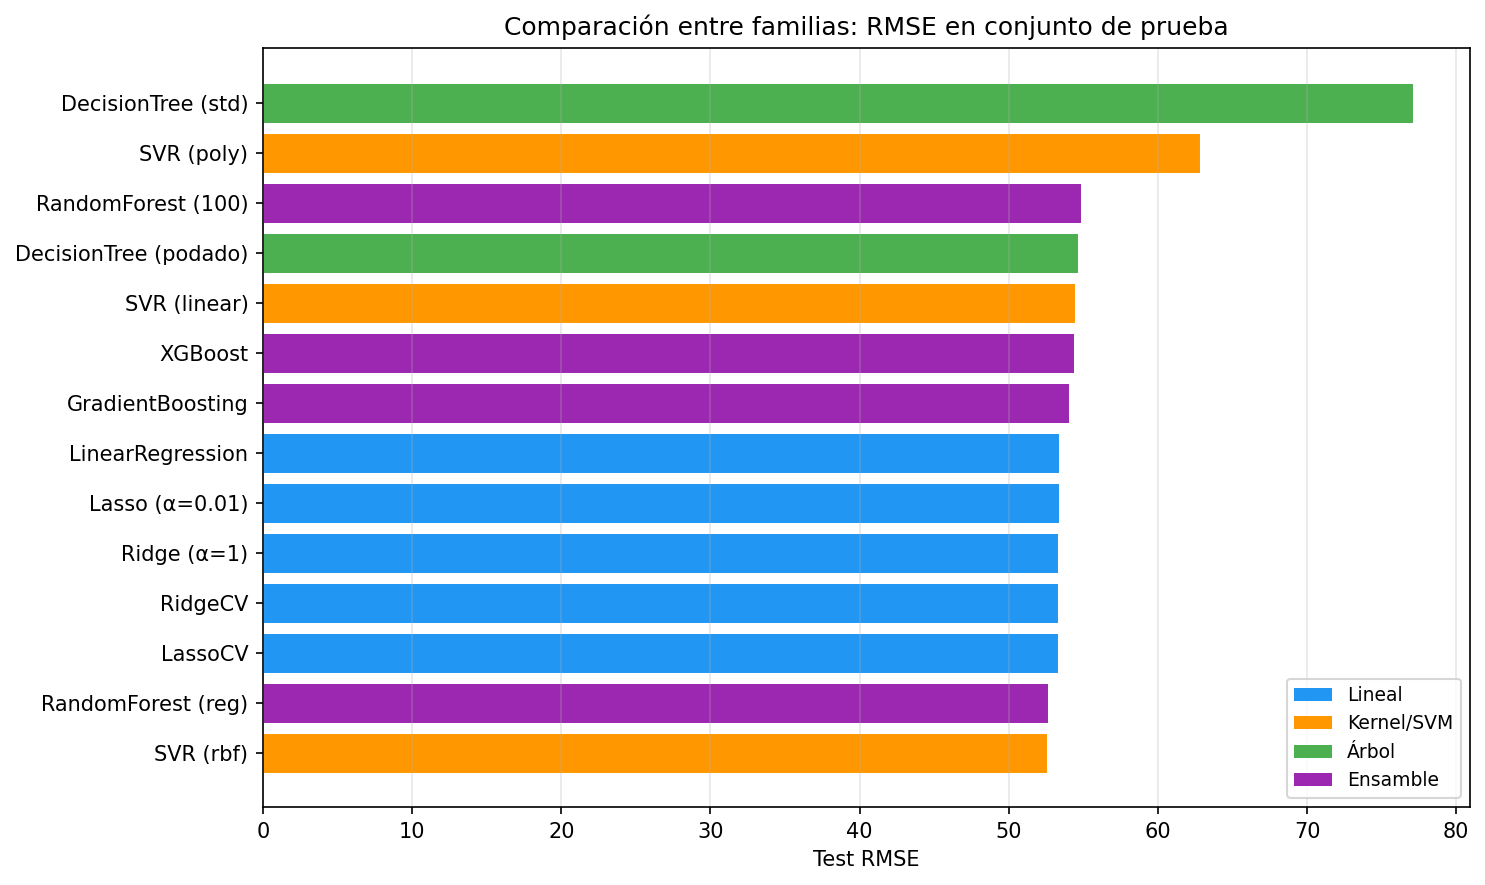
\includegraphics[width=0.92\textwidth]{cross_family_rmse.png}
\caption{Comparación entre familias: RMSE en conjunto de prueba. Los colores representan la familia del algoritmo.}
\label{fig:cf_rmse}
\end{figure}

\begin{figure}[H]
\centering
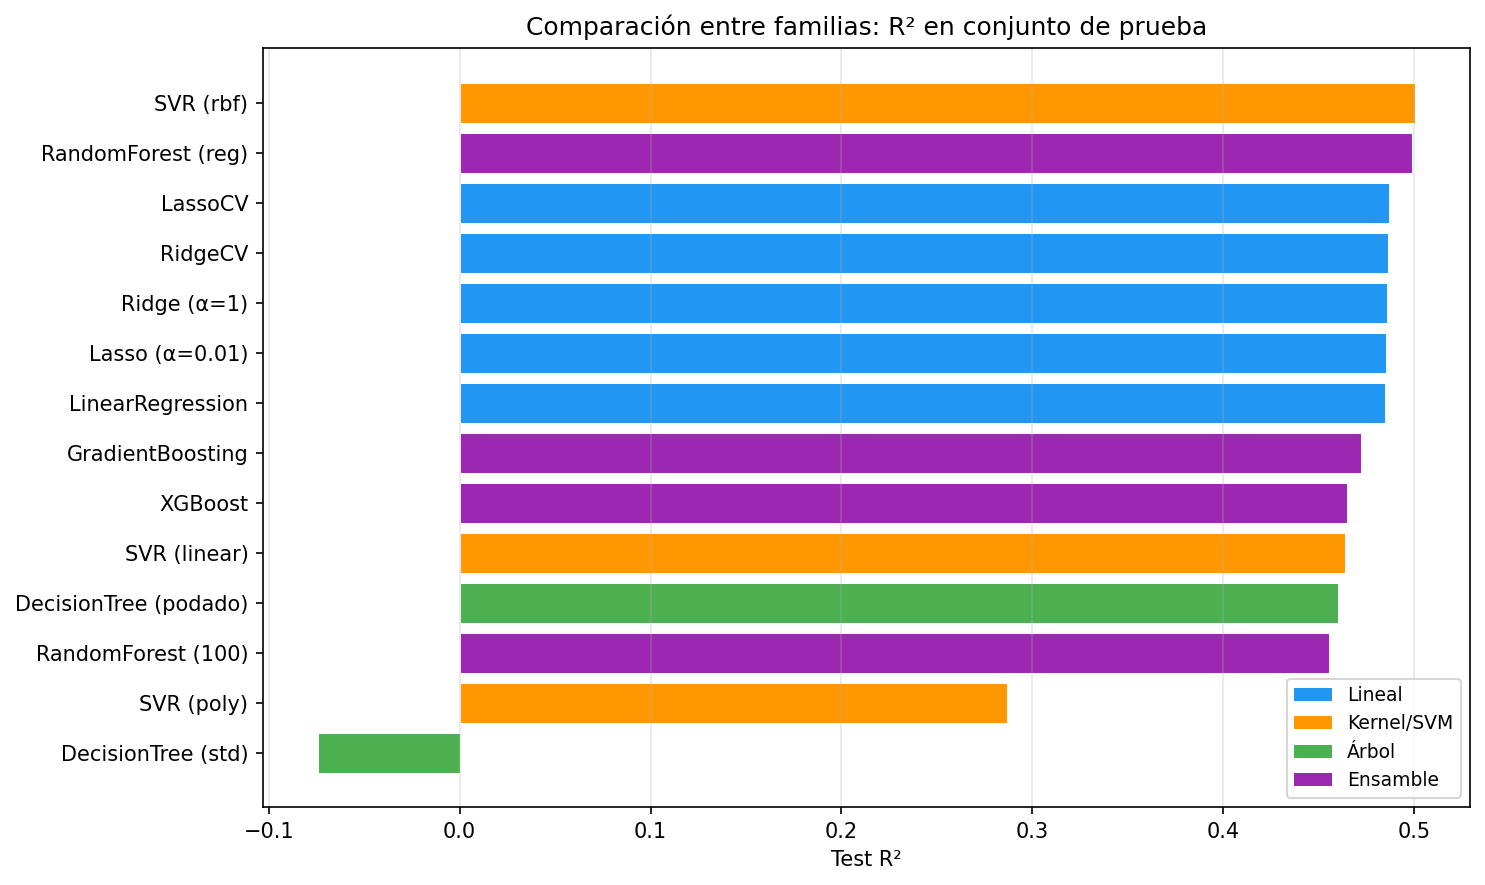
\includegraphics[width=0.92\textwidth]{cross_family_r2.png}
\caption{Comparación entre familias: $R^2$ en conjunto de prueba.}
\label{fig:cf_r2}
\end{figure}

\subsection{Mejor modelo por familia}

La Tabla~\ref{tab:best_per_family} presenta el mejor representante de cada familia según el RMSE promedio de validación cruzada.

\begin{table}[H]
\centering
\caption{Mejor modelo por familia de algoritmo.}
\label{tab:best_per_family}
\begin{tabular}{llrrrr}
\toprule
Familia & Mejor modelo & CV RMSE & Test RMSE & Test MAE & Test $R^2$ \\
\midrule
Lineal & Ridge ($\alpha$=1) & 56.0688 & 53.3182 & 41.5073 & 0.4859 \\
Kernel/SVM & SVR (linear) & 56.2500 & 54.4453 & 41.9288 & 0.4639 \\
Ensamble & XGBoost & 59.3126 & 54.3996 & 42.4433 & 0.4648 \\
Árbol & DT (podado) & 69.6626 & 54.6489 & 43.5694 & 0.4599 \\
\bottomrule
\end{tabular}
\end{table}

\begin{figure}[H]
\centering
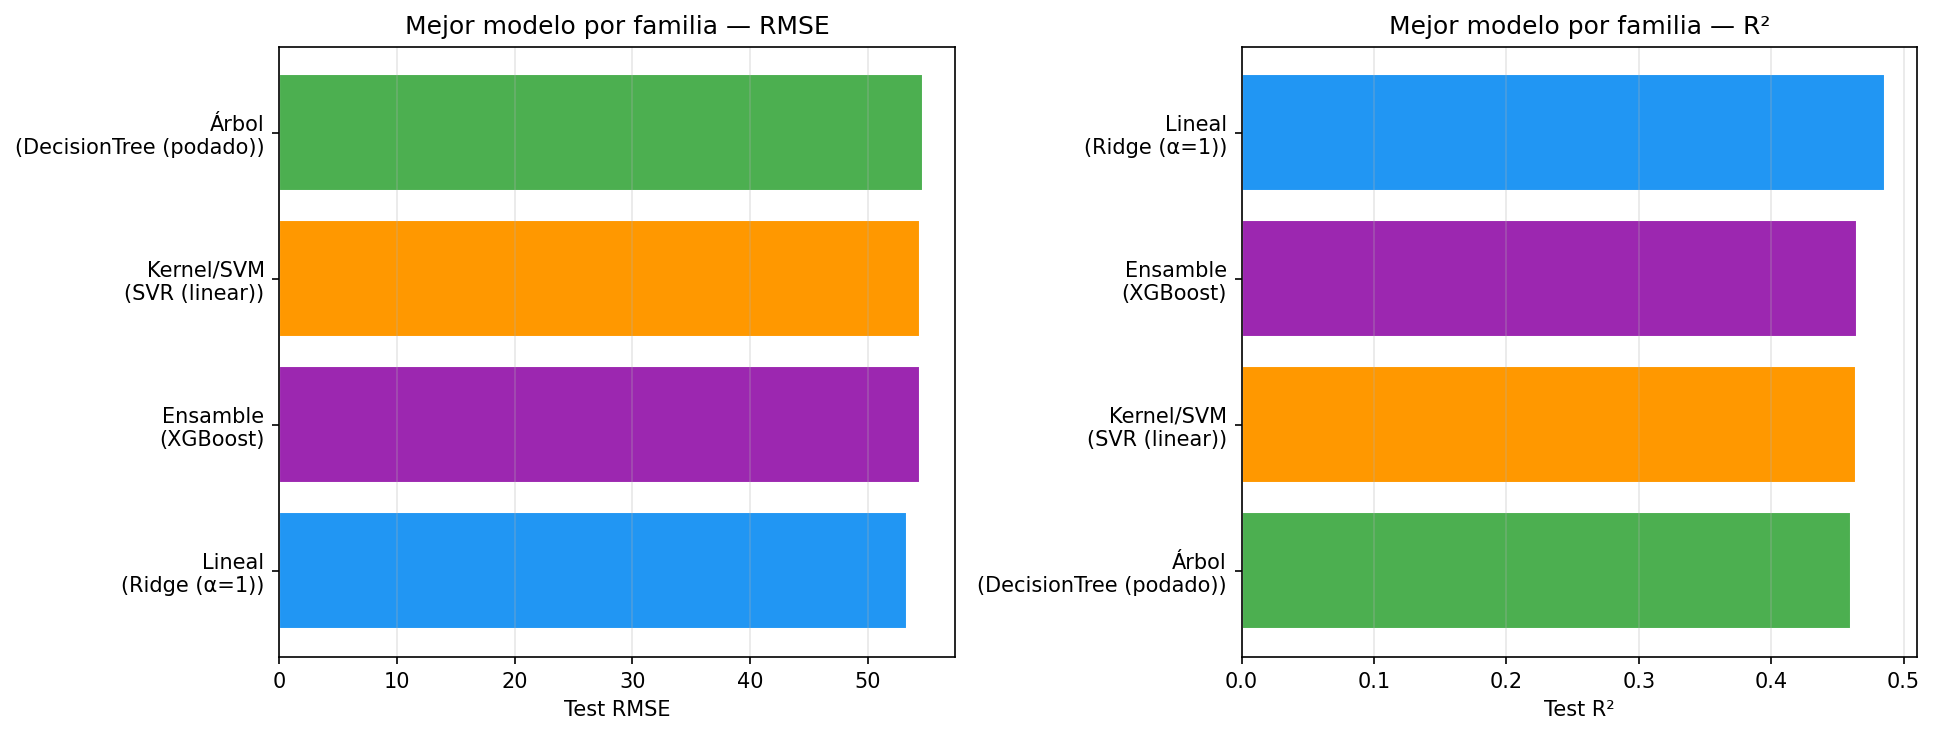
\includegraphics[width=0.95\textwidth]{best_per_family.png}
\caption{Mejor configuración por familia de algoritmo: RMSE y $R^2$ en prueba.}
\label{fig:best_fam}
\end{figure}

\subsection{Estabilidad: validación cruzada frente a prueba}

La Figura~\ref{fig:cv_vs_test} permite identificar modelos con sobreajuste (puntos alejados de la diagonal) y modelos estables (puntos cercanos a ella).

\begin{figure}[H]
\centering
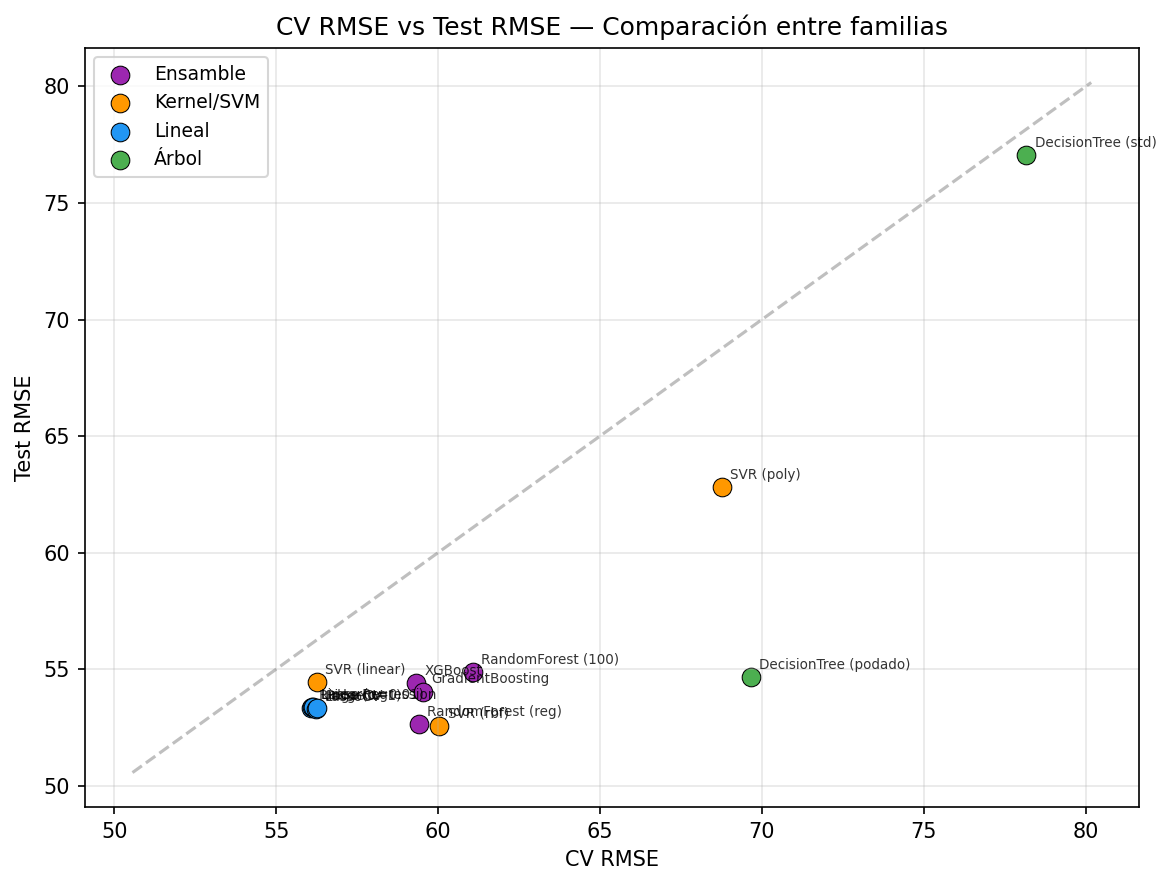
\includegraphics[width=0.85\textwidth]{cv_vs_test_rmse.png}
\caption{RMSE en validación cruzada frente a RMSE en prueba. Los puntos cercanos a la diagonal indican modelos estables.}
\label{fig:cv_vs_test}
\end{figure}

\begin{figure}[H]
\centering
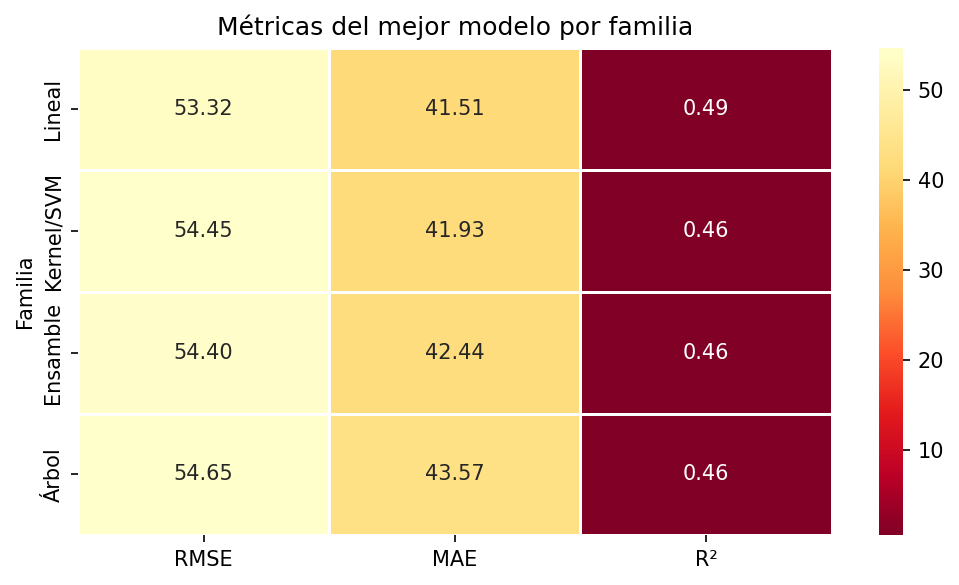
\includegraphics[width=0.7\textwidth]{heatmap_families.png}
\caption{Heatmap de métricas del mejor modelo por familia.}
\label{fig:heatmap_fam}
\end{figure}

\subsection{Análisis del mejor modelo global}

El modelo seleccionado como mejor configuración global fue \textbf{Ridge ($\alpha$=1)}, perteneciente a la familia lineal, con un CV RMSE de 56.0688 y un Test RMSE de 53.3182. Sus métricas completas en el conjunto de prueba fueron:

\begin{table}[H]
\centering
\caption{Métricas del mejor modelo global: Ridge ($\alpha$=1).}
\begin{tabular}{lr}
\toprule
Métrica & Valor \\
\midrule
Test MSE & 2842.83 \\
Test RMSE & 53.3182 \\
Test MAE & 41.5073 \\
Test $R^2$ & 0.4859 \\
\bottomrule
\end{tabular}
\end{table}

\begin{figure}[H]
\centering
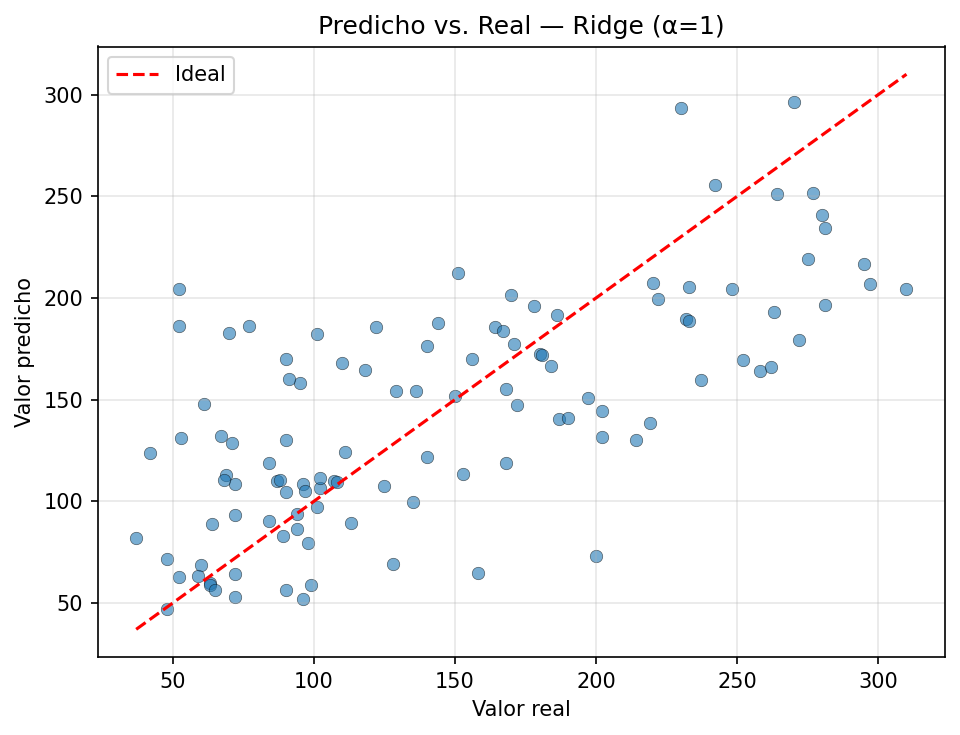
\includegraphics[width=0.72\textwidth]{pred_vs_real_best.png}
\caption{Valores predichos contra valores reales del modelo Ridge ($\alpha$=1).}
\label{fig:pred_real_best}
\end{figure}

\begin{figure}[H]
\centering
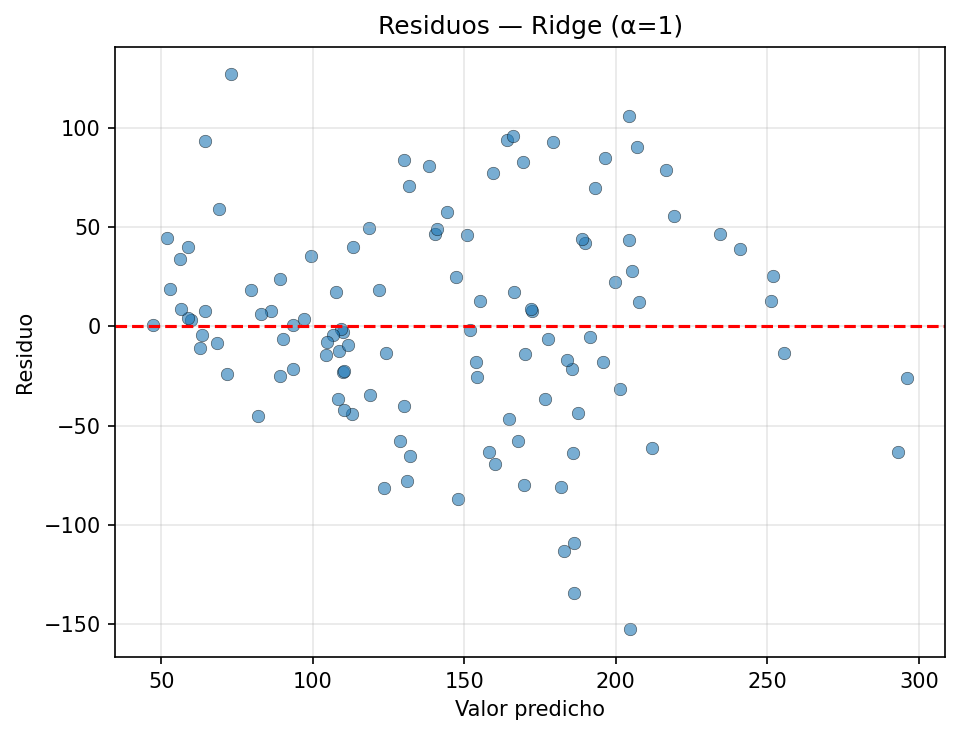
\includegraphics[width=0.72\textwidth]{residuos_best.png}
\caption{Análisis gráfico de residuos del modelo Ridge ($\alpha$=1).}
\label{fig:resid_best}
\end{figure}

\subsection{Discusión entre familias}

\subsubsection{Familia lineal}
Los modelos lineales dominaron la comparación en validación cruzada. Ridge, Lasso y LinearRegression obtuvieron CV RMSE en el rango 56.07--56.27, con Test $R^2$ alrededor de 0.485. Esto indica que la relación entre predictores y variable objetivo en el dataset Diabetes tiene un componente fundamentalmente lineal. La regularización $L_2$ de Ridge ofreció una ligera ventaja por su capacidad de reducir la varianza de los coeficientes ante predictores correlacionados.

\subsubsection{Familia basada en kernels (SVM)}
SVR con kernel lineal se comportó de forma similar a los modelos lineales (CV RMSE 56.25), lo cual es consistente: un kernel lineal es esencialmente una regresión con margen. SVR con kernel RBF obtuvo el \textbf{mejor Test RMSE absoluto} (52.56), pero su CV RMSE fue mayor (60.03), lo que señala menor estabilidad y posible sobreajuste a la partición de prueba. SVR polinómico fue claramente inferior, lo que sugiere que la transformación cúbica no se adapta a la estructura de estos datos.

\subsubsection{Familia basada en árboles}
El árbol sin restricciones presentó sobreajuste severo: CV $R^2$ negativo ($-$0.06) y Test $R^2$ de $-$0.07, indicando un modelo que generaliza peor que la media. La versión podada mejoró drásticamente (Test $R^2$=0.46), confirmando que la regulación mediante \texttt{max\_depth} y \texttt{min\_samples\_leaf} es indispensable. No obstante, un solo árbol no captura suficiente información para competir con los modelos lineales en este dataset.

\subsubsection{Familia de ensambles}
RandomForest regularizado y XGBoost obtuvieron resultados competitivos en prueba (Test $R^2$ de 0.4988 y 0.4648 respectivamente), pero sus CV RMSE fueron superiores a los lineales ($\sim$59). Esto indica que los ensambles capturan relaciones no lineales parciales, pero en un dataset con estructura predominantemente lineal y solo 442 observaciones, la complejidad adicional no se traduce en una ventaja consistente. Es notable que RandomForest regularizado alcanzó un Test $R^2$ cercano a 0.50, sugiriendo que con datasets más grandes o de estructura más compleja podría superar a los modelos lineales.

\subsection{Ventajas y limitaciones por familia}

\begin{table}[H]
\centering
\caption{Ventajas y limitaciones de cada familia en el contexto del dataset Diabetes.}
\resizebox{\textwidth}{!}{%
\begin{tabular}{lp{6.5cm}p{6.5cm}}
\toprule
Familia & Ventajas & Limitaciones \\
\midrule
Lineal & Mejor estabilidad en CV, interpretabilidad directa mediante coeficientes, bajo costo computacional. & Asume linealidad; no captura interacciones ni relaciones no lineales. \\
Kernel/SVM & SVR RBF logra el menor error puntual en prueba; flexibilidad con distintos kernels. & Sensible a hiperparámetros ($C$, $\epsilon$, $\gamma$), menor estabilidad en CV, requiere escalamiento obligatorio. \\
Árbol & Interpretabilidad mediante reglas, manejo natural de no linealidad. & Alto riesgo de sobreajuste sin poda; peor desempeño entre todas las familias. \\
Ensamble & Captura relaciones no lineales, reduce varianza respecto a un árbol individual. & Mayor costo computacional, CV RMSE superior al lineal en este dataset, riesgo de sobreajuste con demasiados estimadores. \\
\bottomrule
\end{tabular}%
}
\end{table}

\subsection{Conclusión de la comparación entre familias}

La comparación entre familias de algoritmos sobre el dataset Diabetes revela que los modelos lineales, particularmente Ridge con regularización $L_2$, representan la mejor opción global al equilibrar estabilidad en validación cruzada, bajo error en prueba e interpretabilidad. Los ensambles y SVR con kernel RBF mostraron capacidad para capturar señales no lineales residuales, pero sin una ventaja consistente bajo validación cruzada. Los árboles de decisión individuales resultaron la familia menos adecuada para este problema.

El criterio de selección prioriza la robustez medida por CV RMSE, dado que el desempeño en una única partición de prueba puede estar sujeto a variabilidad muestral. Bajo este criterio, \textbf{Ridge ($\alpha$=1)} fue el modelo seleccionado como mejor representante global.
